\def\itk{KiSD}
\def\pm{PBSM}
\chapter{实验设计与结果分析}
\label{ch5:experiment}
\section{实验设置}
\subsection{实验环境}
本节对我们提出的解决方案进行了评估。
所有方法均用C++实现,并在一台配备64GB内存、Intel(R) 4210R CPU @ 2.40GHz的CentOS机器上运行。
所有代码和数据集可在GitHub上获取~\cite{code-git-csmtok}。
具体软硬件操作平台如下表\ref{table:setup}所示。
\begin{table}[H]
    \centering
    \caption{实验环境配置}
    \label{table:setup}
    \begin{tabular}{cc}
        \toprule
        描述   & 型号  \\
        \midrule
        CPU处理器 & Intel(R) 4210R CPU @ 2.40GHz\\
        内存 & 64G \\
        硬盘 & 1T\\
        操作系统 & CentOS Linux 7 (Core)\\
        编程语言 & C++ \\
        \bottomrule
    \end{tabular}
\end{table}

\subsection{数据集和评价标准}
\label{ss-sec:dataset}
参考之前的CSM工作~\cite{csm-survey:DBLP:journals/pvldb/SunSLH22,static-sm:DBLP:conf/sigmod/Sun020},我们在实验中使用了五个数据集。
\begin{itemize}
\item Amazon 数据集,一个从亚马逊网站爬取的产品购买网络图。
\item LiveJournal 数据集,包含一个社区网络数据图。
\item Human 数据集,包含一个用于建模蛋白质相互作用网络的大型图。
\item YouTube 数据集,包含一个视频分享网站的社交网络。
\item Orkut 数据集,来自一个免费的在线社交网络,用户在其中互相建立友谊。
\end{itemize}   

具体测试数据集规模如表\ref{table:dataset}所示,表中列出了每个数据集的顶点数,边数,顶点标签数,边标签数,以及图的平均度。
这些数据集的边最大可超过亿,能够有效的展示该算法在处理大规模数据图时的性能表现。通过实验,我们能够全面评估所提出的最终方案在不同规模的数据图中的时间和空间效率。

\begin{table}[H]
    \centering
    \caption{数据集信息描述}
    \label{table:dataset}
    \begin{tabular}{cccccc}
        \toprule
        数据集   & $|V|$  & $|E|$ & $|L(V)|$ & $ |L(E)|$ & $degr(G)=\dfrac{2|E|}{|V|}$\\
        \midrule
        Amazon    & 403,394 & 1,015,000 & 6 & 1 & 5.03     \\ 
        LiveJournal   & 4,847,571 & 30,005,000 & 30 & 1 & 12.38 \\ 
        Human  & 4,674 & 81,282  & 44 & 1 & 34.78   \\ 
        YouTube  & 1,134,890 & 2,015,000 & 25 & 1 & 3.55  \\ 
        Orkut  & 3,072,441 & 117,185,083 & 10 & 1 & 76.28  \\ 
        \bottomrule
    \end{tabular}
\end{table}

请注意,以上数据集中的边是无权的。对于每条边 $(v_1, v_2)$,我们为其分配一个权重,计算方式为:

\[
    \frac{(N(v_1) \cap N(v_2)) + 1}{(N(v_1) \cup N(v_2)) + 1}
\]


结果保留六位小数。该方法生成的边权重反映了顶点邻域的连接程度。
对于上述数据集,我们通过从每个图中随机抽取 $10,000$ 条边来构建相应的更新流。


\textbf{查询图生成}
\label{ss-sec:querygen}

与之前的工作~\cite{csm-turboflux-DBLP:conf/sigmod/KimSHLHCSJ18,csm-symbi-DBLP:journals/pvldb/MinPPGIH21,csm-survey:DBLP:journals/pvldb/SunSLH22}类似,
我们通过从数据图中随机提取子图来生成查询图。
对于每个数据集,我们设置了六种不同的查询大小 ($|E_Q|$):$6$、$8$、$10$、$12$和$14$。
对于每个查询大小,我们提取了10个查询图。
随后,我们评估了不同的 $k$ 值:$100$、$300$、$500$、$700$和$900$。
报告的时间和空间效率结果是通过对相应生成的查询图执行不同算法,并对得到的结果取平均值得到的。

\textbf{对比方法}
本节实验将对我们所提出的算法在上述真实数据集上进行评估,主要涉及以下算法:

(1) Baseline: 第\label{ch3:base-framework}小节中提出的CSM-TopK问题的基础计算框架,并实现利用第k个子图匹配结果作为剪枝上限的基线方案。

(2)MWstar-global:第\ref{mwstar:global}小节中提出的基于全局MWstar索引的面向CSM-TopK问题的算法。

(3)MWstar-both:第\ref{mwstar:local}小节中提出的同时基于全局MWstar和局部MWstar的索引,利用更紧凑的密度上限,解决CSM-TopK问题的算法。

(4) Our-final: 第\label{mwstar:compact-graph}小结中提出的压缩图技术,将它与局部MWstar相结合,形成我们的最终解决方案,并且作为本章实验中的对比算法。

我们将我们的最终方案Our-final(简称为Ours),与现有的具有TopK密度约束的静态子图匹配工作进行比较,包括 \itk\cite{static-topk-Gupta-DBLP:conf/icde/GuptaGYCH14} 和 \pm\cite{static-topk-Chen-DBLP:journals/ijprai/ChenLCTL18}。
此外,我们还将我们的最终方案与几种最先进的CSM方法进行了对比,包含 Graphflow\cite{csm-graphflow-DBLP:conf/sigmod/KankanamgeSMCS17}、Rapidflow\cite{csm-rapidflow-DBLP:journals/pvldb/SunSHL22} 和 CaLiG~\cite{csm-calig-DBLP:journals/pacmmod/YangZZY23}。
需要注意的是,\itk 在处理 LiveJournal 和 YouTube 数据集时,因内存不足而导致无法执行,相关的实验结果标记为“无穷大”。

\section{实验结果分析}
\label{ch5:overall-compare}
\subsection{插入与删除效率对比}
\label{ch5:insertion-deletion}
在本小节中,我们进行了实验以评估我们的算法与其他对比算法在不同数据集上的插入和删除性能。
在该实验中,我们通过固定参数$k$,测试查询图的大小在$6$,$8$,$10$,$12$时的插入平均时间和删除平均时间,如图\ref{fig:time:insertion:fixQuerySize}和图\ref{fig:time:deletion:fixQuerySize}所示;
同样,我们通过固定参数$|E(Q)|$,即查询图的大小,测试参数k的大小在$100$,$300$,$500$,$700$,$900$时的插入平均时间和删除平均时间,如图\ref{fig:time:insertion:fixKSize}和图\ref{fig:time:deletion:fixKSize}所示。

\input{\csmnewFig time_insertion_fixKsize}
\input{\csmnewFig time_insertion_fixQuerySize}
\input{\csmnewFig time_deletion_fixKsize}
\input{\csmnewFig time_deletion_fixQuerySize}

我们通过改变 $k$ 值和查询大小 $|E_Q|$ 来评估在不同数据集下的插入和删除的性能,其中横坐标表示变化的参数,纵坐标表示算法的平均执行时间。


如图~\ref{fig:time:insertion:fixQuerySize} 和图~\ref{fig:time:deletion:fixQuerySize}所示,所有算法在查询图的大小增大时,平均时间均有所增加,
这是因为较大查询图的递归搜索深度通常大于较小查询图,因此所需要的计算时间和存储空间也会增加,从而导致算法的效率有所降低。
如图~\ref{fig:time:insertion:fixKSize} 和图~\ref{fig:time:deletion:fixKSize}所示,其他CSM的解决方法在$k$值不断增加时,对其平均执行时间的影响不大。
这是因为这几种算法均是用于连续子图匹配问题,现有的CSM方法没有基于密度的剪枝,因此它们需要搜索所有新的匹配项以确定前k个匹配结果,且需要对所有的子图匹配结果进行重排序而获取top k的结果。
因此,无论$k$值增加的幅度有多大,其总是维护所有的子图匹配结果,所以其执行时间不随着$k$值的增加而变化。
特别是在Orkut数据集上,Graphflow、RapidFlow和CaLiG的结果非常相似。
而对于\itk 和 \pm,虽然这两种方法有基于密度的剪枝,但是由于它们的索引重建占用了大量的更新时间,也使得不同 $k$ 值之间的差异不太明显。


我们还观察到两个静态TopK方法(\itk 和 \pm)表现最差,因为它们的索引在动态场景下难以更新,在发生更新时需要重新构建索引。
且其索引结构空间占用高,在数据图比较大的情况下,其会因为内存空间耗尽而无法执行。


从图\ref{fig:time:insertion:fixKSize}-图\ref{fig:time:deletion:fixQuerySize}可以看出,我们的算法在插入和删除方面始终优于其他比较解决方案。
随着 $k$ 值的增加,我们的算法的时间成本呈现轻微的上升趋势(见图~\ref{fig:time:insertion:fixKSize} 和图~\ref{fig:time:deletion:fixKSize}),但由于我们的方案比其他方案快2到4个数量级,这一上升趋势几乎可以忽略不计。
更新时间的轻微增加主要是由于随着 $k$ 增大,最小密度下界 $den(g_{min})$ 的松弛(见算法~\ref{alg:find-dense-matches}中的第~\ref{code:g-min-filter}行),从而略微削弱了基于密度的剪枝效果。


\subsection{空间效率对比}
\label{ch5:space}
\input{\csmnewFig space_memory}
我们还评估了我们算法的空间效率。
图~\ref{fig:exp:space:memory}展示了不同方法在不同查询图大小下的内存使用情况。
请注意,在CSM-TopK中,随着参数 $k$ 的变化,空间开销的差异可以忽略不计。
如图~\ref{fig:exp:space:memory}所示,我们的方法在空间效率上明显优于 \itk、\pm、Rapidflow 和 CaLiG。

在LiveJournal,YouTube,Orkut数据集上,\itk、\pm 这两种静态方法都因为耗尽内存而停止,这主要是因为其索引在大规模数据集上的时空复杂度都是指数级别的。
而GraphFlow 在空间使用上方面的性能与我们的方法相似。因为它不维护索引,其对应的空间开销仅来自于维护所有匹配项,由此也能看出我们的索引的轻量级别,其索引仅与查询图的一阶邻居有关,能够达到线性的空间复杂度。


\subsection{索引构建时间对比}
\label{ch5:index-construction}
\begin{figure}[h!]
    \centering
    \resizebox{0.7\linewidth}{!}{
    \includegraphics{\csmnewFig time_index_construct_all.pdf}
    }
    \vspace{-0.01in}
    \caption{索引构建时间  ($|E_Q|=8, k=100$)}
    \label{fig:exp:time:index}
\end{figure}    
我们比较了不同方法的索引构建时间。
从图~\ref{fig:exp:time:index}中可以看出,我们的算法在索引构建时间上比对比算法快2到5个数量级。

而\pm 和 \itk 需要更多时间来构建索引,因为其索引在静态场景下为离线构建,且构建时间较长,而在动态场景下,它们每次更新时都需要重建索引。
Graphflow 没有索引或辅助数据结构,因此不在此实验的范围内。


\subsection{自身对比}
\label{ch5:couterparts}
\begin{figure*}[h!]
    \def\wscorevone{0.30}
    \centering
    % First row - three figures
    \begin{subfigure}[t]{\wscorevone\linewidth}
        \centering
        \resizebox{\linewidth}{!}
        {
            \includegraphics{\csmnewFig time_couterparts_fixQuerySize_amazon.pdf}
        }
        \caption{Amazon}
        \label{fig:time:counterpart:fixQuerySize:amazon}
    \end{subfigure}
    \hspace{1em}
    \begin{subfigure}[t]{\wscorevone\linewidth}
        \centering
        \resizebox{\linewidth}{!}
        {
            \includegraphics{\csmnewFig time_couterparts_fixQuerySize_livejournal.pdf}
        }
        \caption{LiveJournal}
        \label{fig:time:counterpart:fixQuerySize:livejournal}
    \end{subfigure}
    \hspace{1em}
    \begin{subfigure}[t]{\wscorevone\linewidth}
        \centering
        \resizebox{\linewidth}{!}
        {
            \includegraphics{\csmnewFig time_couterparts_fixQuerySize_human.pdf}
        }
        \caption{Human}
        \label{fig:time:counterpart:fixQuerySize:human}
    \end{subfigure}
    
    % Second row - two figures
    \vspace{0.5cm}
    \begin{subfigure}[t]{\wscorevone\linewidth}
        \centering
        \resizebox{\linewidth}{!}
        {
            \includegraphics{\csmnewFig time_couterparts_fixQuerySize_youtube.pdf}
        }
        \caption{YouTube}
        \label{fig:time:counterpart:fixQuerySize:youtube}
    \end{subfigure}
    \hspace{1em}
    \begin{subfigure}[t]{\wscorevone\linewidth}
        \centering
        \resizebox{\linewidth}{!}
        {
            \includegraphics{\csmnewFig time_couterparts_fixQuerySize_orkut.pdf}
        }
        \caption{Orkut}
        \label{fig:time:counterpart:fixQuerySize:orkut}
    \end{subfigure}
    \caption{ 不同$E(Q)$下自身算法效率对比($k=100$)}
    \label{fig:time:counterpart:fixQuerySize}
\end{figure*}
    
    
\input{./exp/newFIg/time_couterparts_fixKSize}


\label{sec:couterparts}
我们将我们提出的四种优化算法进行比较,以展示我们的最终优化策略的有效性。
图 \ref{fig:time:counterpart:fixQuerySize} -图 \ref{fig:time:counterpart:fixKSize} 展示了我们提出的不同算法在不同的 $k$ 值和查询大小 $|E_Q|$ 下的时间开销。
我们可以看到,基于压缩图的最终版本显著优于基于原始图的版本,性能提升了约 $1{\sim}2$ 个数量级。
同时,MWstar-global 和 MWstar-both 的性能明显优于基准方法。
从图 \ref{fig:time:counterpart:fixQuerySize} 到图 \ref{fig:time:counterpart:fixKSize} 可以看出,MWstar-both 的搜索效率明显高于 MWstar-global。
我们可以看到,我们算法的优势在于 MWstar 索引和图压缩策略,将这两者结合形成最终的优化算法,能够将算法的执行效率提升到最高。

\section{案例研究}
\begin{figure}[h!]
    \centering
    \resizebox{0.8\linewidth}{!}{
    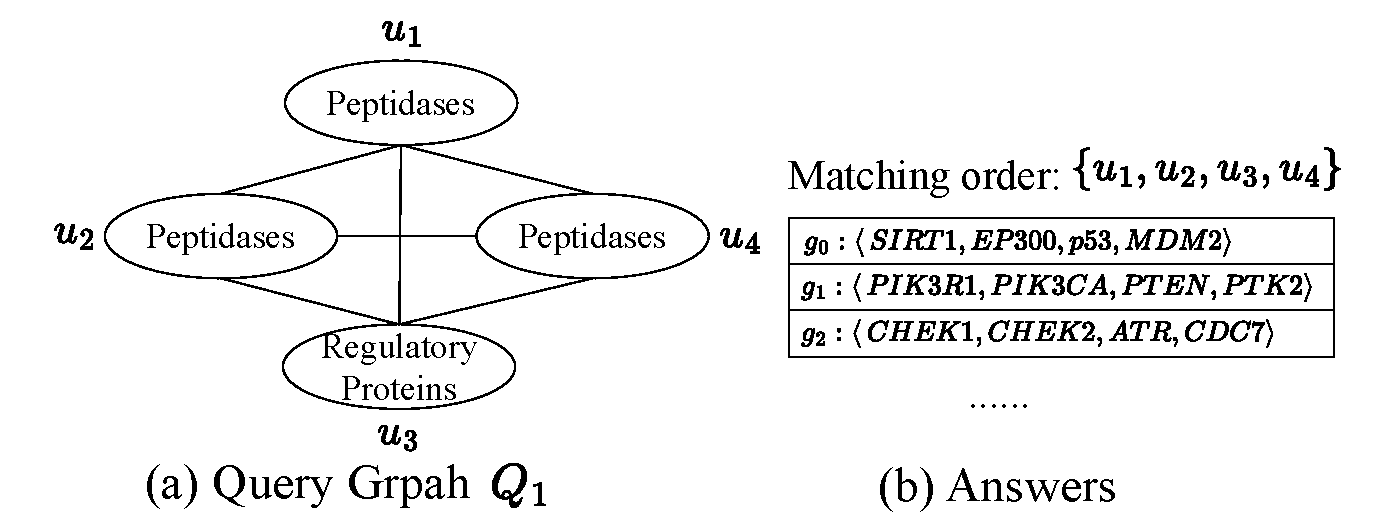
\includegraphics{./exp/newFIg/human_casestudy.pdf}
    }
    \caption{基于蛋白质相互作用网络的案例研究}
    \label{fig:human-caseStudy}
    \end{figure}    
图 \ref{fig:human-caseStudy} 展示了一个查询图 $Q_1$ 及其在蛋白质相互作用网络~\cite{dat-protein} 中的查询结果。
    $Q_1$ 表示由一个调节蛋白和3个肽酶组成的关键结构,边的权重表示相互促进或抑制的程度。
    我们根据边的权重优先排序关系,以识别与相互作用度最高的前 $k$ 个子图。
    在匹配顺序 ${u_1, u_2, u_3, u_4}$ 下,最密集的答案是 $g_0=${$SIRT1$, $EP300$, $p53$, $MDM2$}。
    请注意,$p53$ 是在人类细胞中广泛研究的肿瘤抑制蛋白,而其他三个蛋白激酶表现出强烈的相互作用,并对 $p53$ 产生显著的促进作用,这可能与肿瘤疾病的状态密切相关。
\section{本章小结}
本章详细介绍了我们提出的算法的实验设计与结果分析。
首先介绍了实验环境与配置,包括硬件和软件平台的详细信息、五个真实数据集、查询图的生成方式、以及参与测试的算法。
在实验中,我们通过从数据图中随机抽取子图生成查询图,并对不同查询图大小和不同的$k$值进行了全面测试。
接着,我们对实验结果进行深入分析,通过对比不同算法的时间和空间效率,证明与其他已有的解决方案相比,我们的方案在插入和删除效率上,比其他方案快2-4个数量级,这验证了我们的优化方法在处理大规模数据集时的优势。
同时,我们对比了我们自己提出的四种算法,分别是基线算法、全局MWstar算法、全局与局部MWstar结合的算法以及最终提出的压缩图上的MWstar算法。
实验结果表明,我们的最终算法显著优于基线方法,提升了$1\sim2$个数量级。此外,基于MWstar的全局和局部索引方法也表现出明显的性能优势,尤其是在搜索效率方面,证明了我们算法的有效性和优越性。
最后,我们还给出了CSM-TopK问题在蛋白质相互交互网络上的案例研究,验证了此算法的应用研究价值。